\documentclass{standalone}
\usepackage{tikz}
\usetikzlibrary{patterns, positioning}
\usepackage[sfdefault]{ClearSans} %% option 'sfdefault' activates Clear Sans as the default text font
\usepackage[T1]{fontenc}

\begin{document}
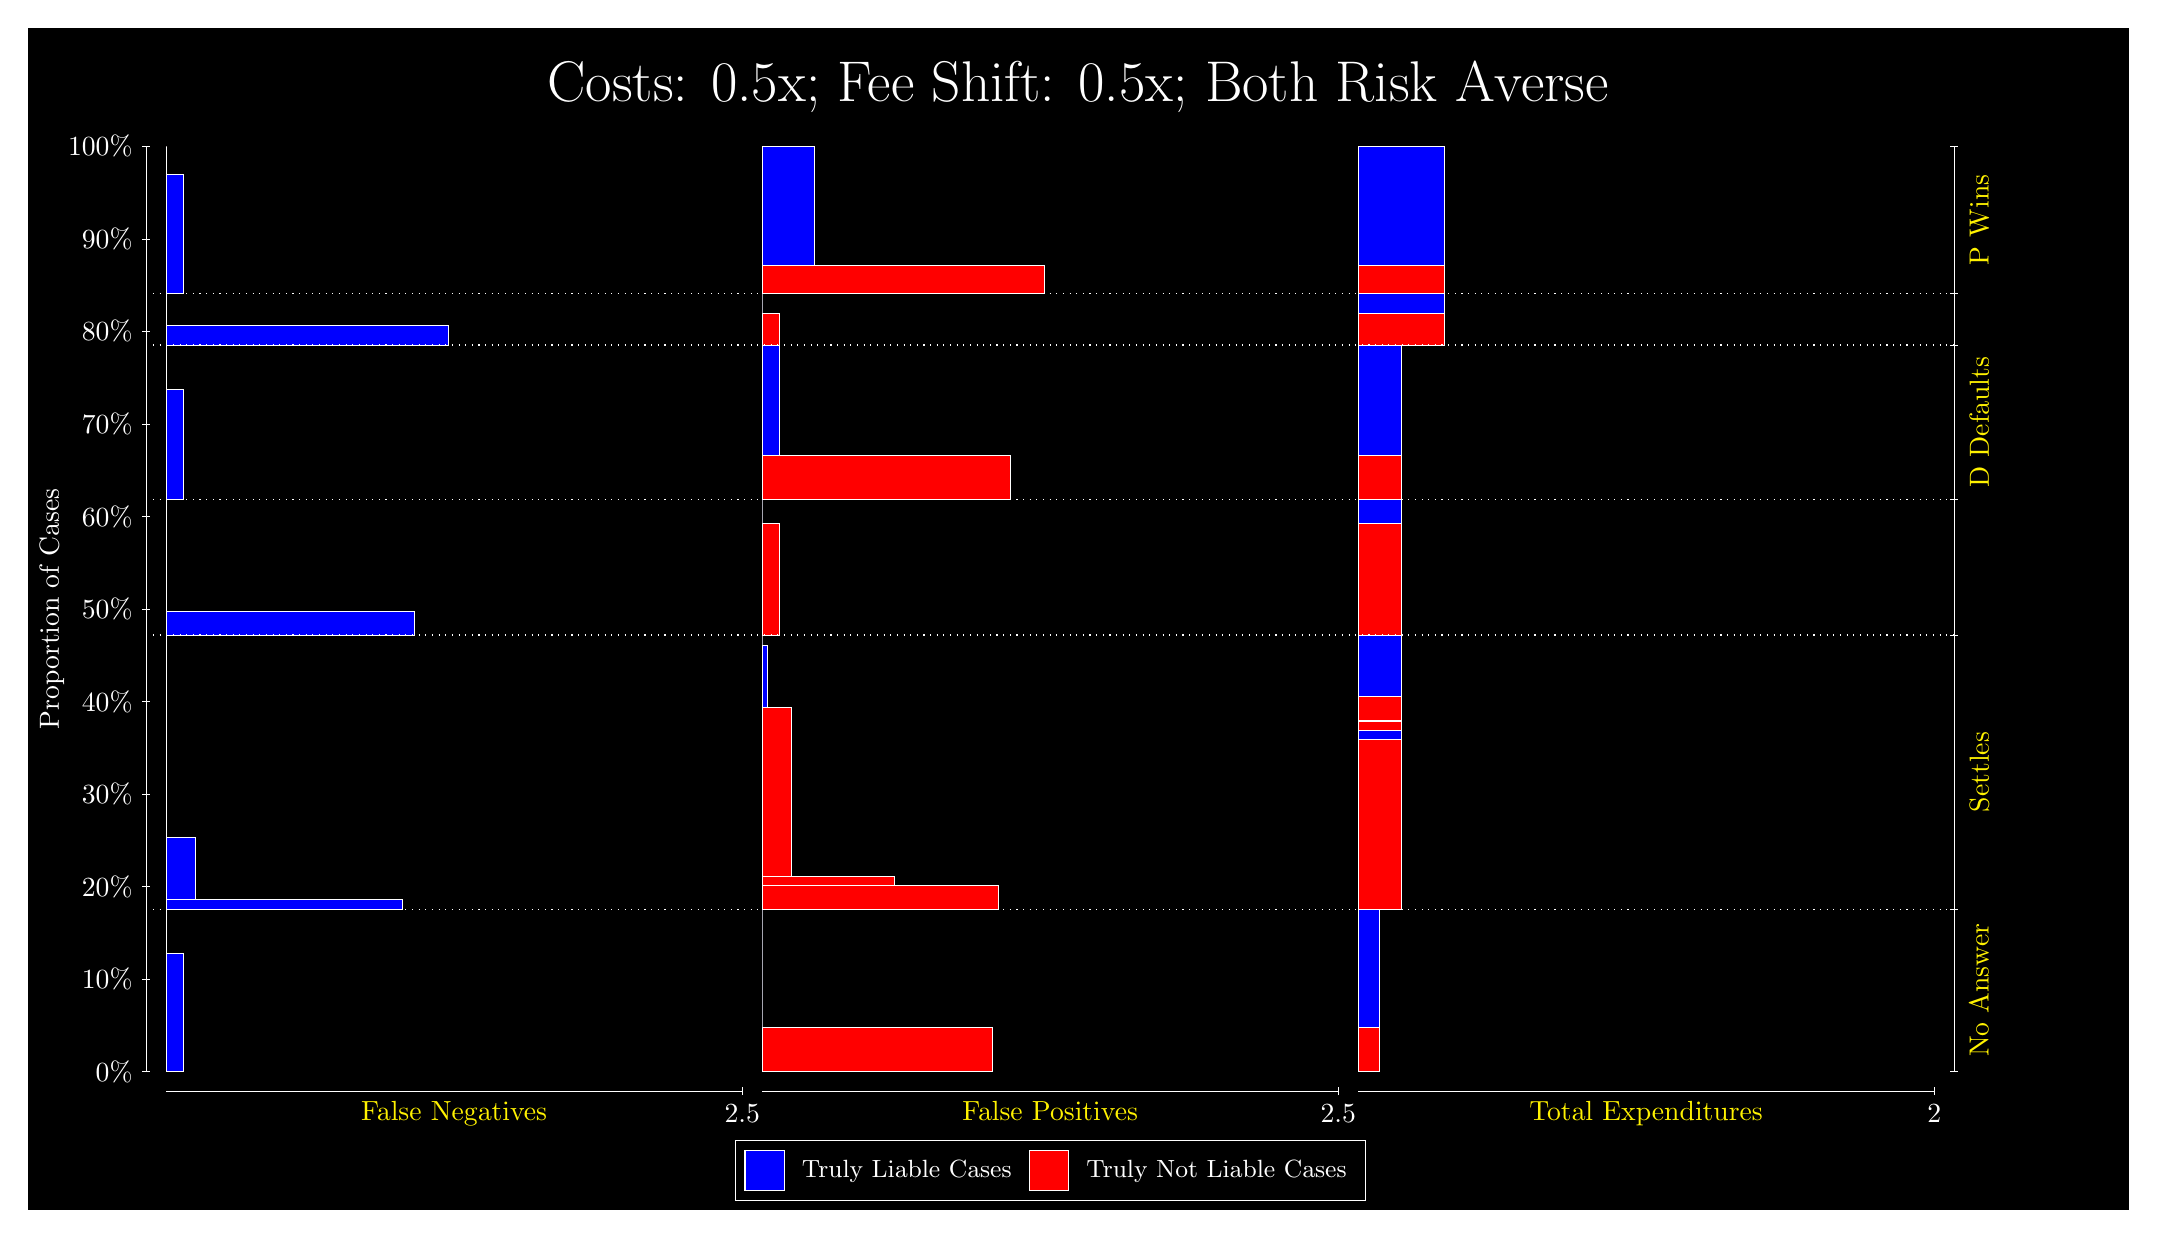
\begin{tikzpicture}
\draw[fill=black] (0,0) rectangle (26.667,15);
\draw[text=white] (0,13.5) rectangle (26.667,15) node[midway] {\huge Costs: 0.5x; Fee Shift: 0.5x; Both Risk Averse};
\draw[white, very thin] (1.5,1.75) -- (1.5,13.5);
\node[rotate=90, text=white, anchor=center] at (0.3, 7.625) {Proportion of Cases};
\draw[white, very thin] (1.45,1.75) -- (1.55,1.75);
\node[text=white, anchor=east] at (1.45, 1.75) {0\%};
\draw[white, very thin] (1.45,2.925) -- (1.55,2.925);
\node[text=white, anchor=east] at (1.45, 2.925) {10\%};
\draw[white, very thin] (1.45,4.1) -- (1.55,4.1);
\node[text=white, anchor=east] at (1.45, 4.1) {20\%};
\draw[white, very thin] (1.45,5.275) -- (1.55,5.275);
\node[text=white, anchor=east] at (1.45, 5.275) {30\%};
\draw[white, very thin] (1.45,6.45) -- (1.55,6.45);
\node[text=white, anchor=east] at (1.45, 6.45) {40\%};
\draw[white, very thin] (1.45,7.625) -- (1.55,7.625);
\node[text=white, anchor=east] at (1.45, 7.625) {50\%};
\draw[white, very thin] (1.45,8.8) -- (1.55,8.8);
\node[text=white, anchor=east] at (1.45, 8.8) {60\%};
\draw[white, very thin] (1.45,9.975) -- (1.55,9.975);
\node[text=white, anchor=east] at (1.45, 9.975) {70\%};
\draw[white, very thin] (1.45,11.15) -- (1.55,11.15);
\node[text=white, anchor=east] at (1.45, 11.15) {80\%};
\draw[white, very thin] (1.45,12.325) -- (1.55,12.325);
\node[text=white, anchor=east] at (1.45, 12.325) {90\%};
\draw[white, very thin] (1.45,13.5) -- (1.55,13.5);
\node[text=white, anchor=east] at (1.45, 13.5) {100\%};

\draw[white, very thin] (24.457,1.75) -- (24.457,13.5);
\draw[white, very thin] (24.407,1.75) -- (24.507,1.75);
\node[anchor=west] at (24.407, 1.75) {};
\draw[white, very thin] (24.407,3.8122) -- (24.507,3.8122);
\node[anchor=west] at (24.407, 3.8122) {};
\draw[white, very thin] (24.407,7.2944) -- (24.507,7.2944);
\node[anchor=west] at (24.407, 7.2944) {};
\draw[white, very thin] (24.407,9.0128) -- (24.507,9.0128);
\node[anchor=west] at (24.407, 9.0128) {};
\draw[white, very thin] (24.407,10.977) -- (24.507,10.977);
\node[anchor=west] at (24.407, 10.977) {};
\draw[white, very thin] (24.407,11.633) -- (24.507,11.633);
\node[anchor=west] at (24.407, 11.633) {};
\draw[white, very thin] (24.407,13.5) -- (24.507,13.5);
\node[anchor=west] at (24.407, 13.5) {};

\draw[white, very thin, fill=blue] (1.75,1.75) rectangle (1.9696,3.2557);
\draw[white, very thin, fill=red] (1.75,3.2557) rectangle (1.75,3.8122);
\draw[white, very thin, fill=blue] (1.75,3.8122) rectangle (4.7507,3.9346);
\draw[white, very thin, fill=blue] (1.75,3.9346) rectangle (3.4333,3.9426);
\draw[white, very thin, fill=blue] (1.75,3.9426) rectangle (2.1159,4.7255);
\draw[white, very thin, fill=red] (1.75,4.7255) rectangle (1.75,7.2944);
\draw[white, very thin, fill=blue] (1.75,7.2944) rectangle (4.8971,7.5922);
\draw[white, very thin, fill=red] (1.75,7.5922) rectangle (1.75,9.0128);
\draw[white, very thin, fill=blue] (1.75,9.0128) rectangle (1.9696,10.41);
\draw[white, very thin, fill=red] (1.75,10.41) rectangle (1.75,10.977);
\draw[white, very thin, fill=blue] (1.75,10.977) rectangle (5.3362,11.229);
\draw[white, very thin, fill=red] (1.75,11.229) rectangle (1.75,11.633);
\draw[white, very thin, fill=blue] (1.75,11.633) rectangle (1.9696,13.142);
\draw[white, very thin, fill=red] (1.75,13.142) rectangle (1.75,13.5);
\draw[white, very thin, fill=red] (9.3189,1.75) rectangle (12.246,2.3065);
\draw[white, very thin, fill=blue] (9.3189,2.3065) rectangle (9.3189,3.8122);
\draw[white, very thin, fill=red] (9.3189,3.8122) rectangle (12.32,4.113);
\draw[white, very thin, fill=red] (9.3189,4.113) rectangle (11.002,4.2286);
\draw[white, very thin, fill=red] (9.3189,4.2286) rectangle (9.6848,6.3811);
\draw[white, very thin, fill=blue] (9.3189,6.3811) rectangle (9.3921,7.1641);
\draw[white, very thin, fill=blue] (9.3189,7.1641) rectangle (9.3189,7.2944);
\draw[white, very thin, fill=red] (9.3189,7.2944) rectangle (9.5384,8.715);
\draw[white, very thin, fill=blue] (9.3189,8.715) rectangle (9.3189,9.0128);
\draw[white, very thin, fill=red] (9.3189,9.0128) rectangle (12.466,9.5795);
\draw[white, very thin, fill=blue] (9.3189,9.5795) rectangle (9.5384,10.977);
\draw[white, very thin, fill=red] (9.3189,10.977) rectangle (9.5384,11.381);
\draw[white, very thin, fill=blue] (9.3189,11.381) rectangle (9.3189,11.633);
\draw[white, very thin, fill=red] (9.3189,11.633) rectangle (12.905,11.991);
\draw[white, very thin, fill=blue] (9.3189,11.991) rectangle (9.9776,13.5);
\draw[white, very thin, fill=red] (16.888,1.75) rectangle (17.162,2.3065);
\draw[white, very thin, fill=blue] (16.888,2.3065) rectangle (17.162,3.8122);
\draw[white, very thin, fill=red] (16.888,3.8122) rectangle (17.437,5.9647);
\draw[white, very thin, fill=blue] (16.888,5.9647) rectangle (17.437,6.0871);
\draw[white, very thin, fill=red] (16.888,6.0871) rectangle (17.437,6.2027);
\draw[white, very thin, fill=blue] (16.888,6.2027) rectangle (17.437,6.2107);
\draw[white, very thin, fill=red] (16.888,6.2107) rectangle (17.437,6.5115);
\draw[white, very thin, fill=blue] (16.888,6.5115) rectangle (17.437,7.2944);
\draw[white, very thin, fill=red] (16.888,7.2944) rectangle (17.437,8.715);
\draw[white, very thin, fill=blue] (16.888,8.715) rectangle (17.437,9.0128);
\draw[white, very thin, fill=red] (16.888,9.0128) rectangle (17.437,9.5795);
\draw[white, very thin, fill=blue] (16.888,9.5795) rectangle (17.437,10.977);
\draw[white, very thin, fill=red] (16.888,10.977) rectangle (17.986,11.381);
\draw[white, very thin, fill=blue] (16.888,11.381) rectangle (17.986,11.633);
\draw[white, very thin, fill=red] (16.888,11.633) rectangle (17.986,11.991);
\draw[white, very thin, fill=blue] (16.888,11.991) rectangle (17.986,13.5);
\draw[white, dotted] (1.5,3.8122) -- (24.457,3.8122);
\draw[white, dotted] (1.5,7.2944) -- (24.457,7.2944);
\draw[white, dotted] (1.5,9.0128) -- (24.457,9.0128);
\draw[white, dotted] (1.5,10.977) -- (24.457,10.977);
\draw[white, dotted] (1.5,11.633) -- (24.457,11.633);
\draw[white, very thin] (1.75,1.5) -- (9.0689,1.5);
\node[text=yellow, anchor=north] at (5.4094, 1.5) {False Negatives};
\draw[white, very thin] (9.0689,1.45) -- (9.0689,1.55);
\node[text=white, anchor=north] at (9.0689, 1.45) {2.5};

\draw[white, very thin] (9.3189,1.5) -- (16.638,1.5);
\node[text=yellow, anchor=north] at (12.978, 1.5) {False Positives};
\draw[white, very thin] (16.638,1.45) -- (16.638,1.55);
\node[text=white, anchor=north] at (16.638, 1.45) {2.5};

\draw[white, very thin] (16.888,1.5) -- (24.207,1.5);
\node[text=yellow, anchor=north] at (20.547, 1.5) {Total Expenditures};
\draw[white, very thin] (24.207,1.45) -- (24.207,1.55);
\node[text=white, anchor=north] at (24.207, 1.45) {2};

\node[text=yellow, centered, rotate=90] at (24.777, 2.7811) {No Answer};
\node[text=yellow, centered, rotate=90] at (24.777, 5.5533) {Settles};

\node[text=yellow, centered, rotate=90] at (24.777, 9.9949) {D Defaults};

\node[text=yellow, centered, rotate=90] at (24.777, 12.566) {P Wins};

\draw (12.978300999999998,1.5) node[draw=none] (baseCoordinate) {};
\begin{scope}[align=center]
        \matrix[scale=0.5, draw=white, below=0.5cm of baseCoordinate, nodes={draw}, column sep=0.1cm]{
            \node[rectangle, draw, minimum width=0.5cm, minimum height=0.5cm, fill=blue] {}; &
            \node[draw=none, font=\small, text=white] (B) {Truly Liable Cases}; &
            \node[rectangle, draw, minimum width=0.5cm, minimum height=0.5cm, fill=red] {}; &
            \node[draw=none, font=\small, text=white] (B) {Truly Not Liable Cases}; \\
            };
\end{scope}

\end{tikzpicture}
\end{document}